% Standalone figure for the Statistical Mechanics notes.
% Build: pdflatex binary-lens.tex  (or run build.sh in this folder)
\documentclass[11pt,tikz,border=2pt]{standalone}
\usepackage{amsmath,amssymb}
\usetikzlibrary{arrows.meta, positioning}
\begin{document}
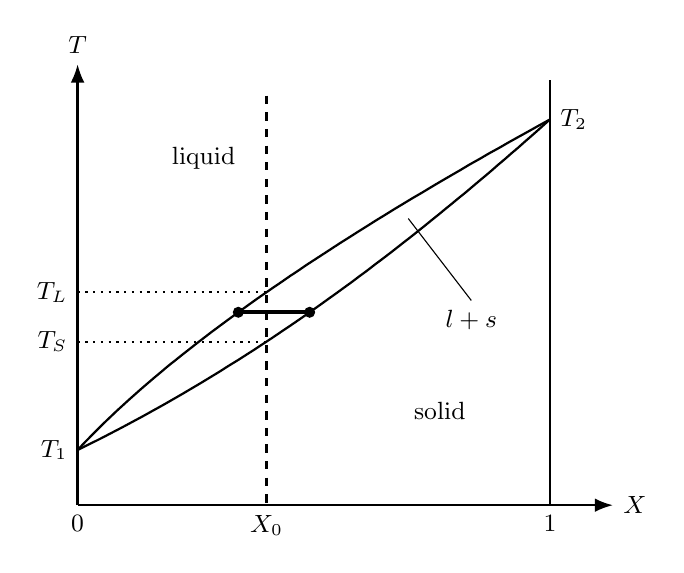
\begin{tikzpicture}[font=\small, >=Latex, line width=0.8pt]
    % axes: x = 6X, y = 7(T - 0.9); T_1 = 1.0, T_2 = 1.6,
    % l_1/k_B = 1.3, l_2/k_B = 2.1
    \draw[->] (0,0) -- (6.8,0) node[right] {$X$};
    \draw[->] (0,0) -- (0,5.6) node[above] {$T$};
    \draw (6,0) -- (6,5.4);
    \node[below] at (0,0) {$0$};
    \node[below] at (6,0) {$1$};
    % liquidus X^l(T)
    \draw[domain=1.0005:1.5995, smooth, samples=60, variable=\t]
        plot ({6*(1-exp(1.3*(1/\t-1)))/(exp(2.1*(1/\t-1/1.6))-exp(1.3*(1/\t-1)))},
              {7*(\t-0.9)});
    % solidus X^s(T)
    \draw[domain=1.0005:1.5995, smooth, samples=60, variable=\t]
        plot ({6*exp(2.1*(1/\t-1/1.6))*(1-exp(1.3*(1/\t-1)))/(exp(2.1*(1/\t-1/1.6))-exp(1.3*(1/\t-1)))},
              {7*(\t-0.9)});
    % melting points
    \node[left] at (0,0.7) {$T_1$};
    \node[right] at (6,4.9) {$T_2$};
    % cooling path at X_0 = 0.4 and tie line at T = 1.25
    \draw[dashed] (2.4,5.2) -- (2.4,0) node[below] {$X_0$};
    \draw[line width=1.6pt] (2.041,2.45) -- (2.947,2.45);
    \fill (2.041,2.45) circle (2pt);
    \fill (2.947,2.45) circle (2pt);
    \draw[dotted] (0,2.705) node[left] {$T_L$} -- (2.4,2.705);
    \draw[dotted] (0,2.077) node[left] {$T_S$} -- (2.4,2.077);
    % region labels
    \node at (1.6,4.4) {liquid};
    \node at (4.6,1.2) {solid};
    \draw[line width=0.4pt] (4.2,3.64) -- (5.0,2.6) node[below] {$l+s$};
\end{tikzpicture}
\end{document}
